% !TEX TS-program = pdflatex
% !TEX encoding = UTF-8 Unicode

% This is a simple template for a LaTeX document using the "article" class.
% See "book", "report", "letter" for other types of document.

\documentclass[11pt]{article} % use larger type; default would be 10pt

\usepackage[utf8]{inputenc} % set input encoding (not needed with XeLaTeX)

%%% Examples of Article customizations
% These packages are optional, depending whether you want the features they provide.
% See the LaTeX Companion or other references for full information.

%%% PAGE DIMENSIONS
\usepackage{geometry} % to change the page dimensions
\geometry{a4paper} % or letterpaper (US) or a5paper or....
% \geometry{margin=2in} % for example, change the margins to 2 inches all round
% \geometry{landscape} % set up the page for landscape
%   read geometry.pdf for detailed page layout information
\addtolength{\topmargin}{-.875in}
\addtolength{\textheight}{1.75in}

\usepackage{graphicx} % support the \includegraphics command and options

% \usepackage[parfill]{parskip} % Activate to begin paragraphs with an empty line rather than an indent

%%% PACKAGES
\usepackage{booktabs} % for much better looking tables
\usepackage{array} % for better arrays (eg matrices) in maths
\usepackage{paralist} % very flexible & customisable lists (eg. enumerate/itemize, etc.)
\usepackage{verbatim} % adds environment for commenting out blocks of text & for better verbatim
\usepackage{subfig} % make it possible to include more than one captioned figure/table in a single float
% These packages are all incorporated in the memoir class to one degree or another...

%%% HEADERS & FOOTERS
\usepackage{fancyhdr} % This should be set AFTER setting up the page geometry
\pagestyle{fancy} % options: empty , plain , fancy
\renewcommand{\headrulewidth}{0pt} % customise the layout...
\lhead{}\chead{}\rhead{}
\lfoot{}\cfoot{\thepage}\rfoot{}

%%% SECTION TITLE APPEARANCE
\usepackage{sectsty}
\allsectionsfont{\sffamily\mdseries\upshape} % (See the fntguide.pdf for font help)
% (This matches ConTeXt defaults)

%%% ToC (table of contents) APPEARANCE
\usepackage[nottoc,notlof,notlot]{tocbibind} % Put the bibliography in the ToC
\usepackage[titles,subfigure]{tocloft} % Alter the style of the Table of Contents
\renewcommand{\cftsecfont}{\rmfamily\mdseries\upshape}
\renewcommand{\cftsecpagefont}{\rmfamily\mdseries\upshape} % No bold!

%%% END Article customizations

%%% The "real" document content comes below...

\title{PROTEST: Manual Annotation Guidelines\\Version 1.0}
%\author{The Author}
%/\date{9 February 2016} % Activate to display a given date or no date (if empty),
         % otherwise the current date is printed 

\begin{document}
\maketitle

\section{Introduction}
\textit{PROTEST} is a pronoun test suite, designed to enable researchers to evaluate their Machine Translation (MT) systems on the specific task of pronoun translation. The test suite comprises:
\begin{itemize}
  \item A set of hand-selected pronoun tokens, categorised according to a number of features
  \item An automatic evaluation script
  \item A graphical user interface (GUI), which may be used to:
  \begin{itemize}
    \item Browse the translations of the set of hand-selected pronoun tokens
    \item Manually annotate those pronoun tokens which cannot be evaluated automatically
  \end{itemize}
\end{itemize}

\section{Getting started}
To run the PROTEST manual annotation tool:
\begin{enumerate}
  \item Open a terminal window
  \item Navigate to the PROTEST directory
  \item Run the command: \textbf{sh gui.sh}
\end{enumerate}

\noindent
This will open the \textbf{PROTEST Browser window} (see Figure \ref{fig:BrowserWindow}).

\begin{figure}[h!]
    \centering
    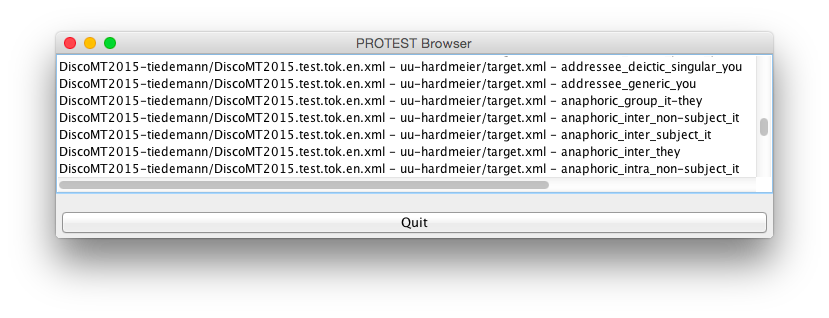
\includegraphics[width=0.99\textwidth]{PROTESTBrowserWindow.png}
    \caption{PROTEST Browser window}
    \label{fig:BrowserWindow}
\end{figure}

Select on the system output + pronoun category combination entry that you wish to annotate. This will open the \textbf{Manual Annotation window} (see Figure \ref{fig:AnnotationWindow}).

\begin{figure}[h!]
    \centering
    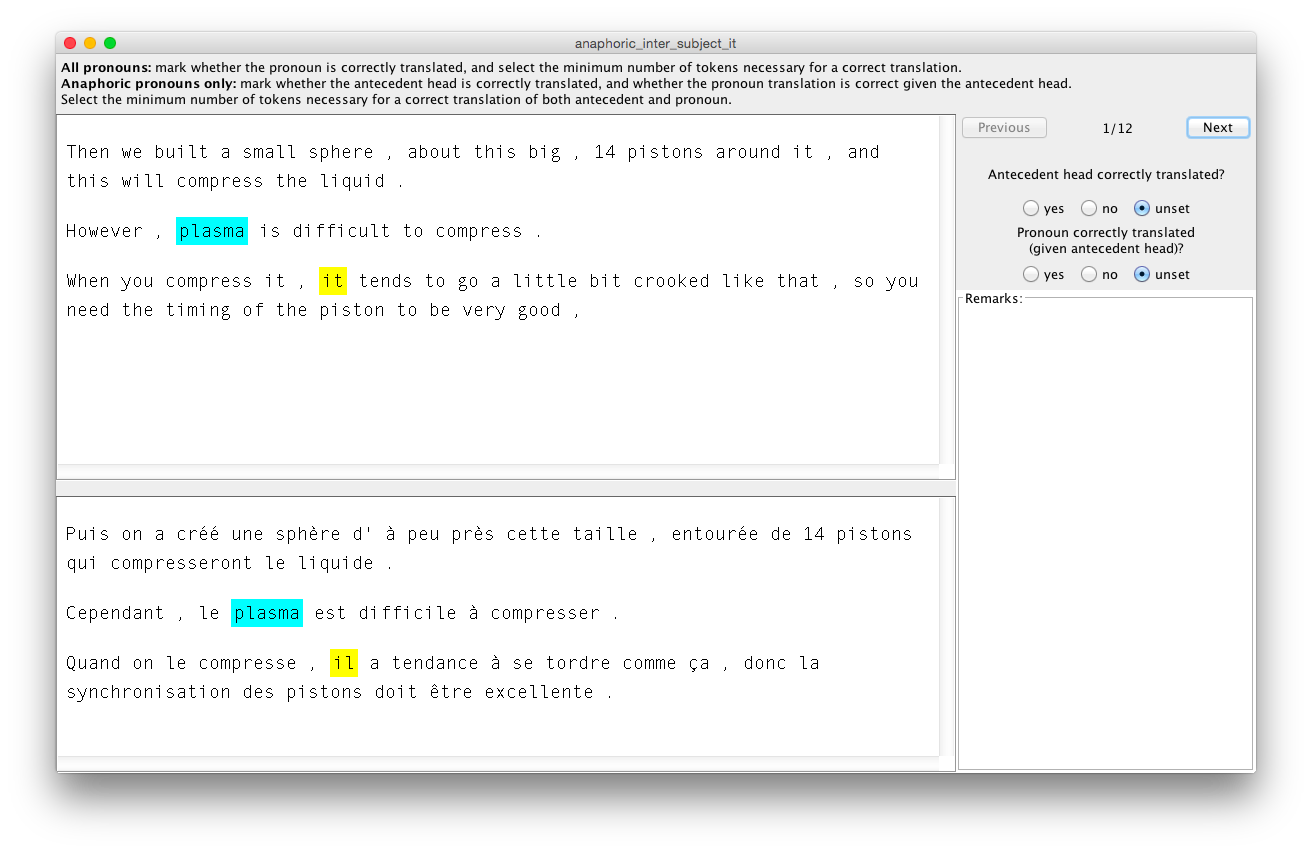
\includegraphics[width=0.99\textwidth]{ManualAnnotationWindow.png}
    \caption{Manual Annotation window}
    \label{fig:AnnotationWindow}
\end{figure}

Follow the annotation guidelines in Section \ref{AnnotationGuidelines} to complete the annotations. Your annotations will be saved automatically when you use the \textbf{Previous} and \textbf{Next} buttons to navigate between pronoun tokens in the set, or when you close the \textbf{Manual Annotation window}.

To exit the PROTEST manual annotation tool, click on the \textbf{Quit} button in the \textbf{PROTEST Browser window}.

\section{Annotation Guidelines}
\label{AnnotationGuidelines}
Select a batch of pronoun tokens from the \textbf{PROTEST Browser window}, for the desired MT system and pronoun category. The \textbf{Manual Annotation window} will appear. For each highlighted pronoun token, read the source-language text (top frame) and the MT system output (bottom frame). Consider the translation of the source-language pronoun token that is highlighted in yellow. If the source-language pronoun was translated by the MT system, the translation (consisting of one or more tokens) in the MT system output will also be highlighted in yellow.

Complete the annotation of each pronoun instance using the following guidelines:


\subsection{General Guidelines: All Pronouns}

\begin{itemize}
  \item Answer the question: ``Pronoun Correctly Translated?'' using the ``yes/no'' options in the \textbf{annotation panel} in the top right-hand corner of the \textbf{Manual Annotation window}
  \begin{itemize}
    \item You should answer this question for all source-language pronouns, whether or not they are translated by the MT system
    \item If a source-language pronoun is left untranslated by the MT system, use the ``yes/no'' options to mark whether this is correct/incorrect
    \item If you are unsure, you may use the default ``unset'' option and complete the annotation later. Please use the \textbf{remarks box} on the right-hand side of the \textbf{Manual Annotation window} to record any notes that may be useful to you later on
    \item You may come across incorrect translations. If you believe that it is possible to assess the translation of the pronoun independently of the remainder of the translation output, you should annotate the example as normal. If not, you should leave the example un-annotated and add a comment to the \textbf{remarks box}
    \item If the pronoun is present in the translation output but is not highlighted (i.e. a bad alignment), do not attempt to annotate the example. Instead, add a comment to the \textbf{remarks box}
    \item Note: if the pronoun is anaphoric, follow the guidelines in Section \ref{AnaphoricGuidelines}
  \end{itemize}
  \item Select the minimum number of yellow highlighted tokens that constitutes a correct translation of the source-language pronoun. To select a token, click on it. The token highlight will change to orange, indicating that it has been selected. You can select as many highlighted tokens as are required. It is not possible to select tokens that do not have a yellow highlight
  \item Please use the \textbf{remarks box} to record any issues that you would like to discuss, e.g. relating to any difficulties or problems that you encounter during the annotation of a given pronoun
  \item Once you have completed the annotation of the current pronoun instance, move to the next one using the \textbf{Next} button in the top right hand corner of the \textbf{Manual Annotation window}
  \begin{itemize}
    \item If the annotations are conflicting, for example if you have indicated that the pronoun is correctly translated but none of the translated tokens has been selected, a warning will appear. You may choose to make a correction, or proceed to the next pronoun instance
  \end{itemize}
\end{itemize}


\subsection{Anaphoric Pronouns Only}
\label{AnaphoricGuidelines}

If the pronoun is anaphoric, you will need to consider both the translation of the antecedent head and the pronoun. The \textit{head} of the source-language pronoun's \textit{antecedent} will be highlighted in light blue. If the antecedent head has been translated by the MT system, the translation (consisting of one or more tokens) in the MT system output will also be highlighted in light blue.

\begin{itemize}
  \item First, answer the question: ``Antecedent Correctly Translated?'' using the ``yes/no'' options in the \textbf{annotation panel} in the top right-hand corner of the \textbf{Manual Annotation window}
  \begin{itemize}
    \item If the pronoun or the antecedent head are present in the translation output but is not highlighted (i.e. a bad alignment), do not attempt to annotate the example. Instead, add a comment to the \textbf{remarks box}
  \end{itemize}  
  \item Select the minimum number of blue highlighted tokens that constitutes a correct translation of the source-language antecedent head. To select a token, click on it. The token highlight will change to a darker shad of blue, indicating that it has been selected. You can select as many highlighted tokens as are required. It is not possible to select tokens that do not have a blue highlight
  \item Second, answer the question: ``Pronoun Correctly Translated (given antecedent)?'' using the ``yes/no'' options in the \textbf{annotation panel}
  \begin{itemize}
    \item A correctly translated pronoun is one that \textit{is compatible} with the translation of the antecedent head, regardless of whether the antecedent is translated correctly
  \end{itemize}
  \item Select the minimum number of yellow highlighted tokens that constitutes a correct translation of the source-language pronoun (given the antecedent)
\end{itemize}


\section{Conflicting Annotations}
There are a number of scenarios which give rise to conflicting annotations:
\begin{itemize}
  \item All pronouns:
  \begin{itemize}
    \item Pronoun is marked as correct, but no tokens are selected in the translation output
    \item Tokens are selected in the translation output of the pronoun, but the pronoun is not marked as correct
  \end{itemize}
  \item Anaphoric pronouns only:
  \begin{itemize}
    \item Antecedent is marked as correct, but no tokens are selected in the translation output
    \item Tokens are selected in the translation output of the antecedent, but the antecedent is not marked as correct 
  \end{itemize}
\end{itemize}

In the case of anaphoric pronouns, conflicts may exist in the annotation of the pronoun, its antecedent, or both.


\end{document}
